\chapter{Ergebnisse}
\label{chapter:results}

In diesem Kapitel werden die Resultate der angewandten linearen Regressionsanalyse 
zur Vorhersage der Druckfestigkeit von Beton dargestellt. 
Die Analyse berücksichtigt sowohl die geschätzten Koeffizienten des linearen Modells 
als auch verschiedene Evaluierungsmetriken wie den mittleren absoluten Fehler (MAE), 
den mittleren quadratischen Fehler (MSE) sowie die Bestimmtheitsmaße ($R^2$) 
für Trainings- und Testdaten. Diese Metriken liefern Aufschluss über die Güte des Modells 
und die Präzision der Vorhersagen. Zunächst werden die Koeffizienten 
des linearen Modells auf herkömmliche Weise interpretiert. Anschließend wird gezeigt, 
wie SHAP-Werte eine tiefere und detailliertere Analyse ermöglichen.

\section{Lineares Regressionmodell}

Die Koeffizienten des Modells, die in Tabelle \ref{tab:model-coefficients} 
aufgeführt sind, zeigen, wie stark sich eine Einheitänderung jedes unabhängigen Merkmals 
auf die Beton-Druckfestigkeit auswirkt, unter der Vorraussetzung, dass alle anderen 
Merkmale null sind. 

Positive Koeffizienten deuten auf eine Erhöhung der Beton-Druckfestigkeit 
bei Zunahme der Variablen hin, während negative Koeffizienten eine Verringerung anzeigen. 
Der Intercept-Wert repräsentiert die geschätzte Beton-Druckfestigkeit, 
wenn alle unabhängigen Variablen den Wert Null annehmen. 

Daraus ergibt sich zusammen mit Gleichung \ref{eq:reg-model} die Regressionsgerade für das Modell.

\begin{table}[!h]
    \caption{Koeffizienten des linearen Regressionsmodells}
    \begin{tabularx}{\textwidth}{Xr}
    \toprule
    Merkmal ($\beta_j$) & Koeffizient \\
    \midrule
    Intercept ($\beta_0$) & 4.36596 \\
    cement & 0.75091 \\
    blast & 0.06610 \\
    ash & 0.02683 \\
    water & -0.92315 \\
    superplasticizer & 0.06410 \\
    coarse & 0.08554 \\
    fine &  -0.31901 \\
    age & 0.29090 \\
    \bottomrule
    \end{tabularx}
    \label{tab:model-coefficients}
    \\ Quelle: Eigene Darstellung, \ref{linreg}.
\end{table}

Die Modellmetriken, dargestellt in Tabelle \ref{tab:model-metrics}, 
geben Auskunft über die Vorhersagegenauigkeit und die Anpassungsgüte des Modells. 
Der MAE und RMSE liefern dabei Informationen über die durchschnittliche Größe 
der Fehler in den Vorhersagen, und die $R^2$-Werte zeigen, wie gut das Modell die Varianz 
der Zielvariable erklärt.

\begin{table}[!h]
    \caption{Modellmetriken des linearen Regressionsmodells}
    \begin{tabularx}{\textwidth}{Xr}
    \toprule
    Metrik & Wert \\
    \midrule
    Mean Absolute Error (MAE) & 0.19 \\
    Mean Squared Error (MSE) & 0.06 \\
    Root Mean Squared Error (RMSE) & 0.24 \\
    Training Score (R²) & 0.7852 \\
    Test Score (R²) & 0.8155 \\
    \bottomrule
    \end{tabularx}
    \label{tab:model-metrics}
    \\ Quelle: Eigene Darstellung, \ref{linreg}.
\end{table}

Darüber hinaus wurden die tatsächlichen gegen die vorhergesagten Werte
in Abbildung \ref{pic:residuals} visualisiert, die eine allgemeine Einschätzung der 
Modellgenauigkeit ermöglicht. Ein weiterer wichtiger Aspekt sind die Residuen des Modells. 
Die Residuen, also die Differenzen zwischen den tatsächlichen und vorhergesagten Werten, 
sollten idealerweise zufällig um Null verteilt sein und keine Muster aufweisen, 
die auf eine Verletzung der Modellannahmen hindeuten könnten.

\begin{figure}[!h]
    \caption{Residuenanalyse: Beziehung zwischen Vorhersagen und Abweichungen.}
    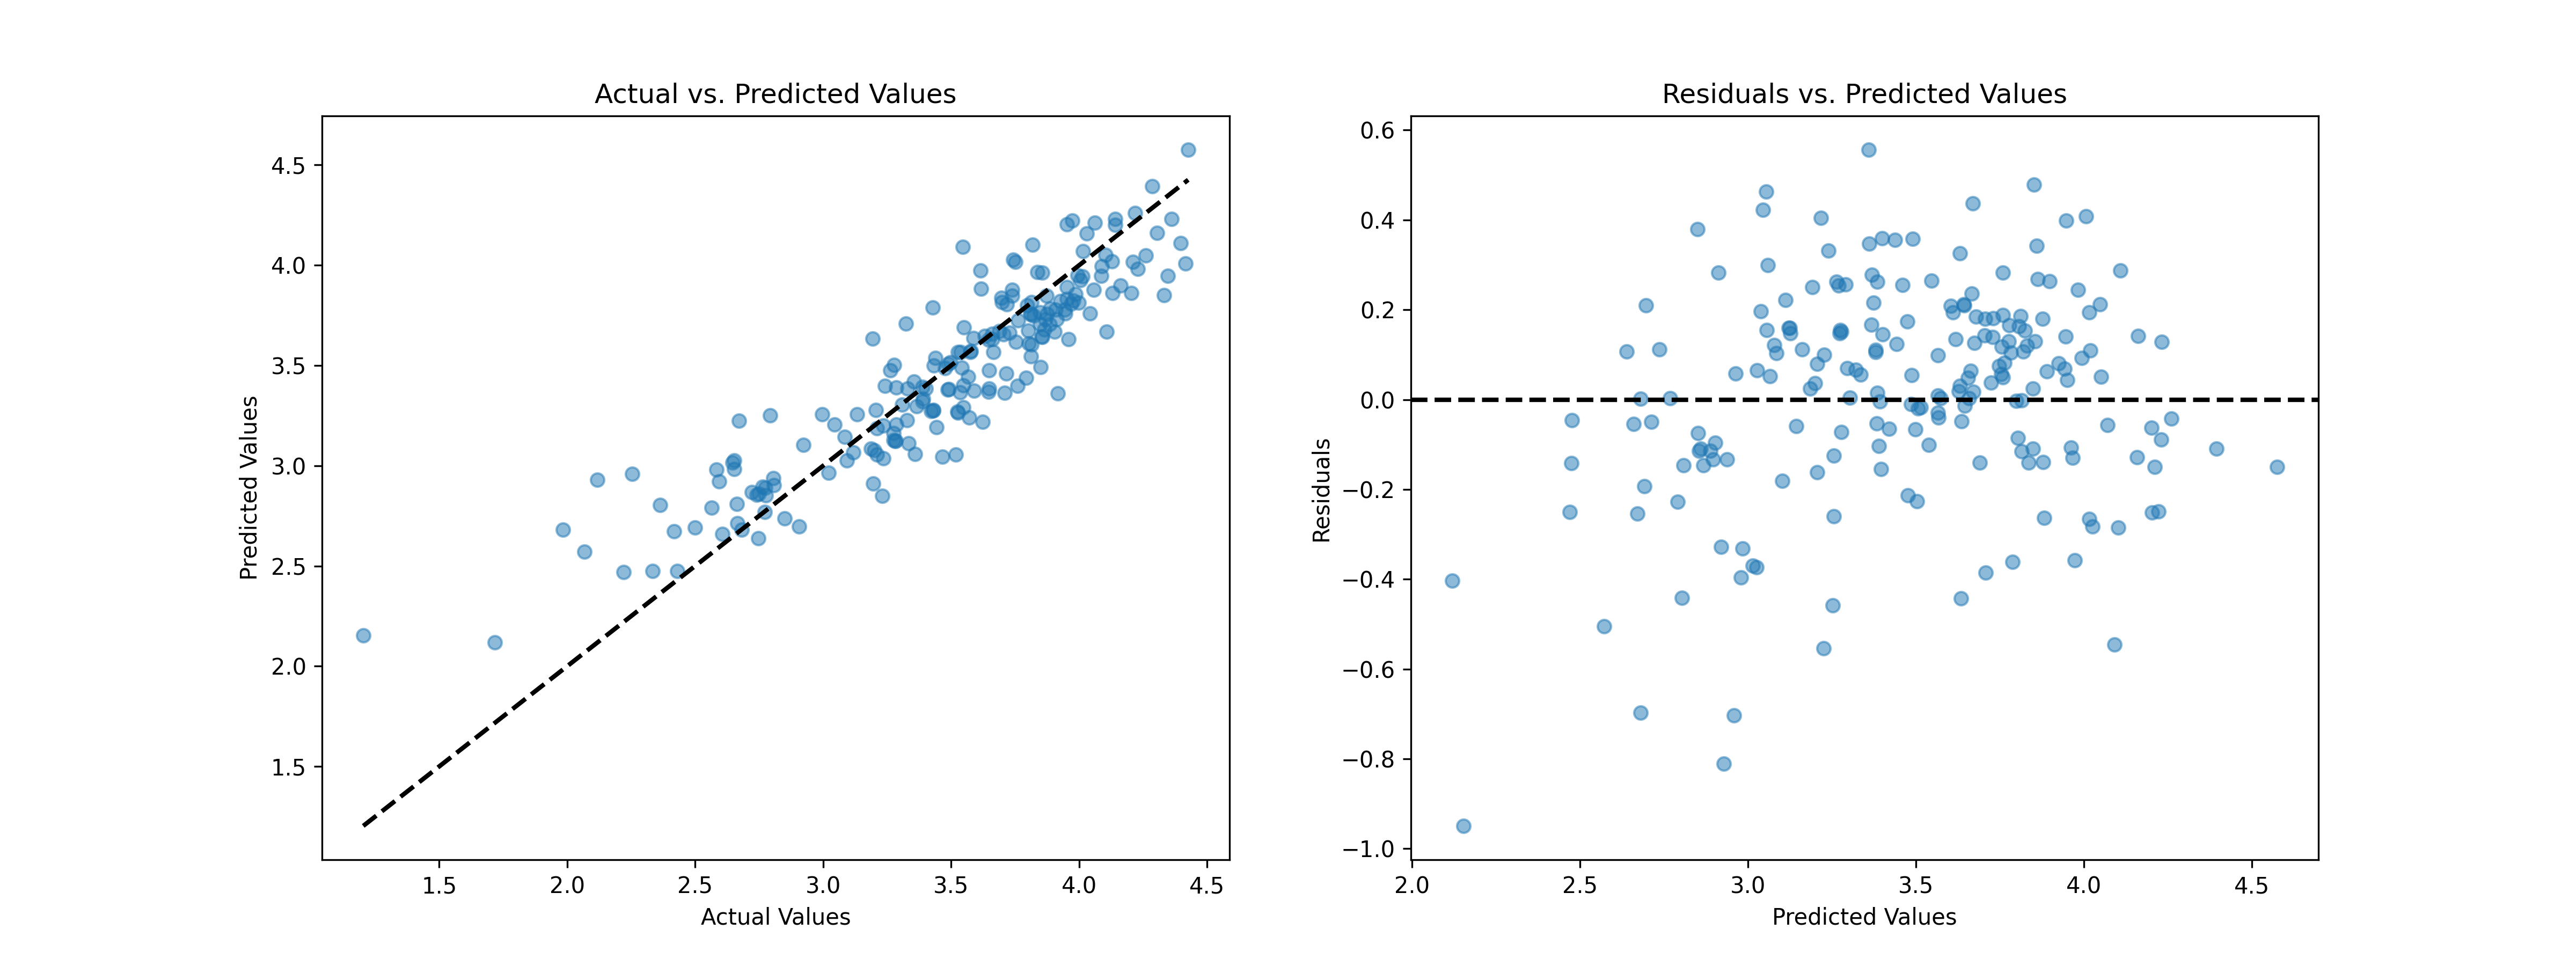
\includegraphics[width=1\textwidth]{../scripts/images/residuals.png}
    Quelle: Eigene Darstellung, \ref{linreg}.
    \label{pic:residuals}
\end{figure}


\section{Interpretation der Koeffizienten \& Permutation Feature Importance}

In diesem Abschnitt wird die herkömmliche Interpretation der Modellkoeffizienten genauer betrachtet. 
Die Koeffizienten eines linearen Modells repräsentieren die Änderung der abhängigen Variable (in diesem Fall die Druckfestigkeit von Beton) 
für eine Einheitänderung der unabhängigen Variablen, unter der Annahme, dass alle anderen Variablen konstant gehalten werden.

Es ist wichtig zu betonen, dass diese Koeffizienten eine bedingte Assoziation beschreiben. 
Das bedeutet, sie quantifizieren die Variation der Druckfestigkeit, wenn eine bestimmte unabhängige Variable 
verändert wird, während alle anderen unabhängigen Variablen konstant gehalten werden. 
Diese Interpretation berücksichtigt die Wechselwirkungen zwischen den verschiedenen unabhängigen Variablen im Modell.

Es ist entscheidend zu verstehen, dass die Koeffizienten nicht als marginale Beiträge betrachtet werden sollten. 
Das bedeutet, sie beschreiben nicht die Beziehung zwischen den Variablen unabhängig von anderen Einflussfaktoren. 
Stattdessen zeigen sie, wie sich die Druckfestigkeit ändert, wenn eine bestimmte unabhängige Variable variiert wird, 
ährend alle anderen konstant gehalten werden.

Abbildung \ref{pic:coef} zeigt die Koeffizienten des Regressionsmodells. Die Stärke des Einflusses einer 
unabhängigen Variable auf die abhängige Variable hängt von der Größe der Merkmalsausprägung ab. 
Ob ein bestimmtes Merkmal einen großen oder kleinen Einfluss auf die abhängige Variable hat, hängt
von den spezifischen Werten der Merkmale und der Streuung der Merkmalsausprägungen ab. 

\begin{figure}[!h]
    \caption{Koeffizienten des linearen Regressionsmodells.}
    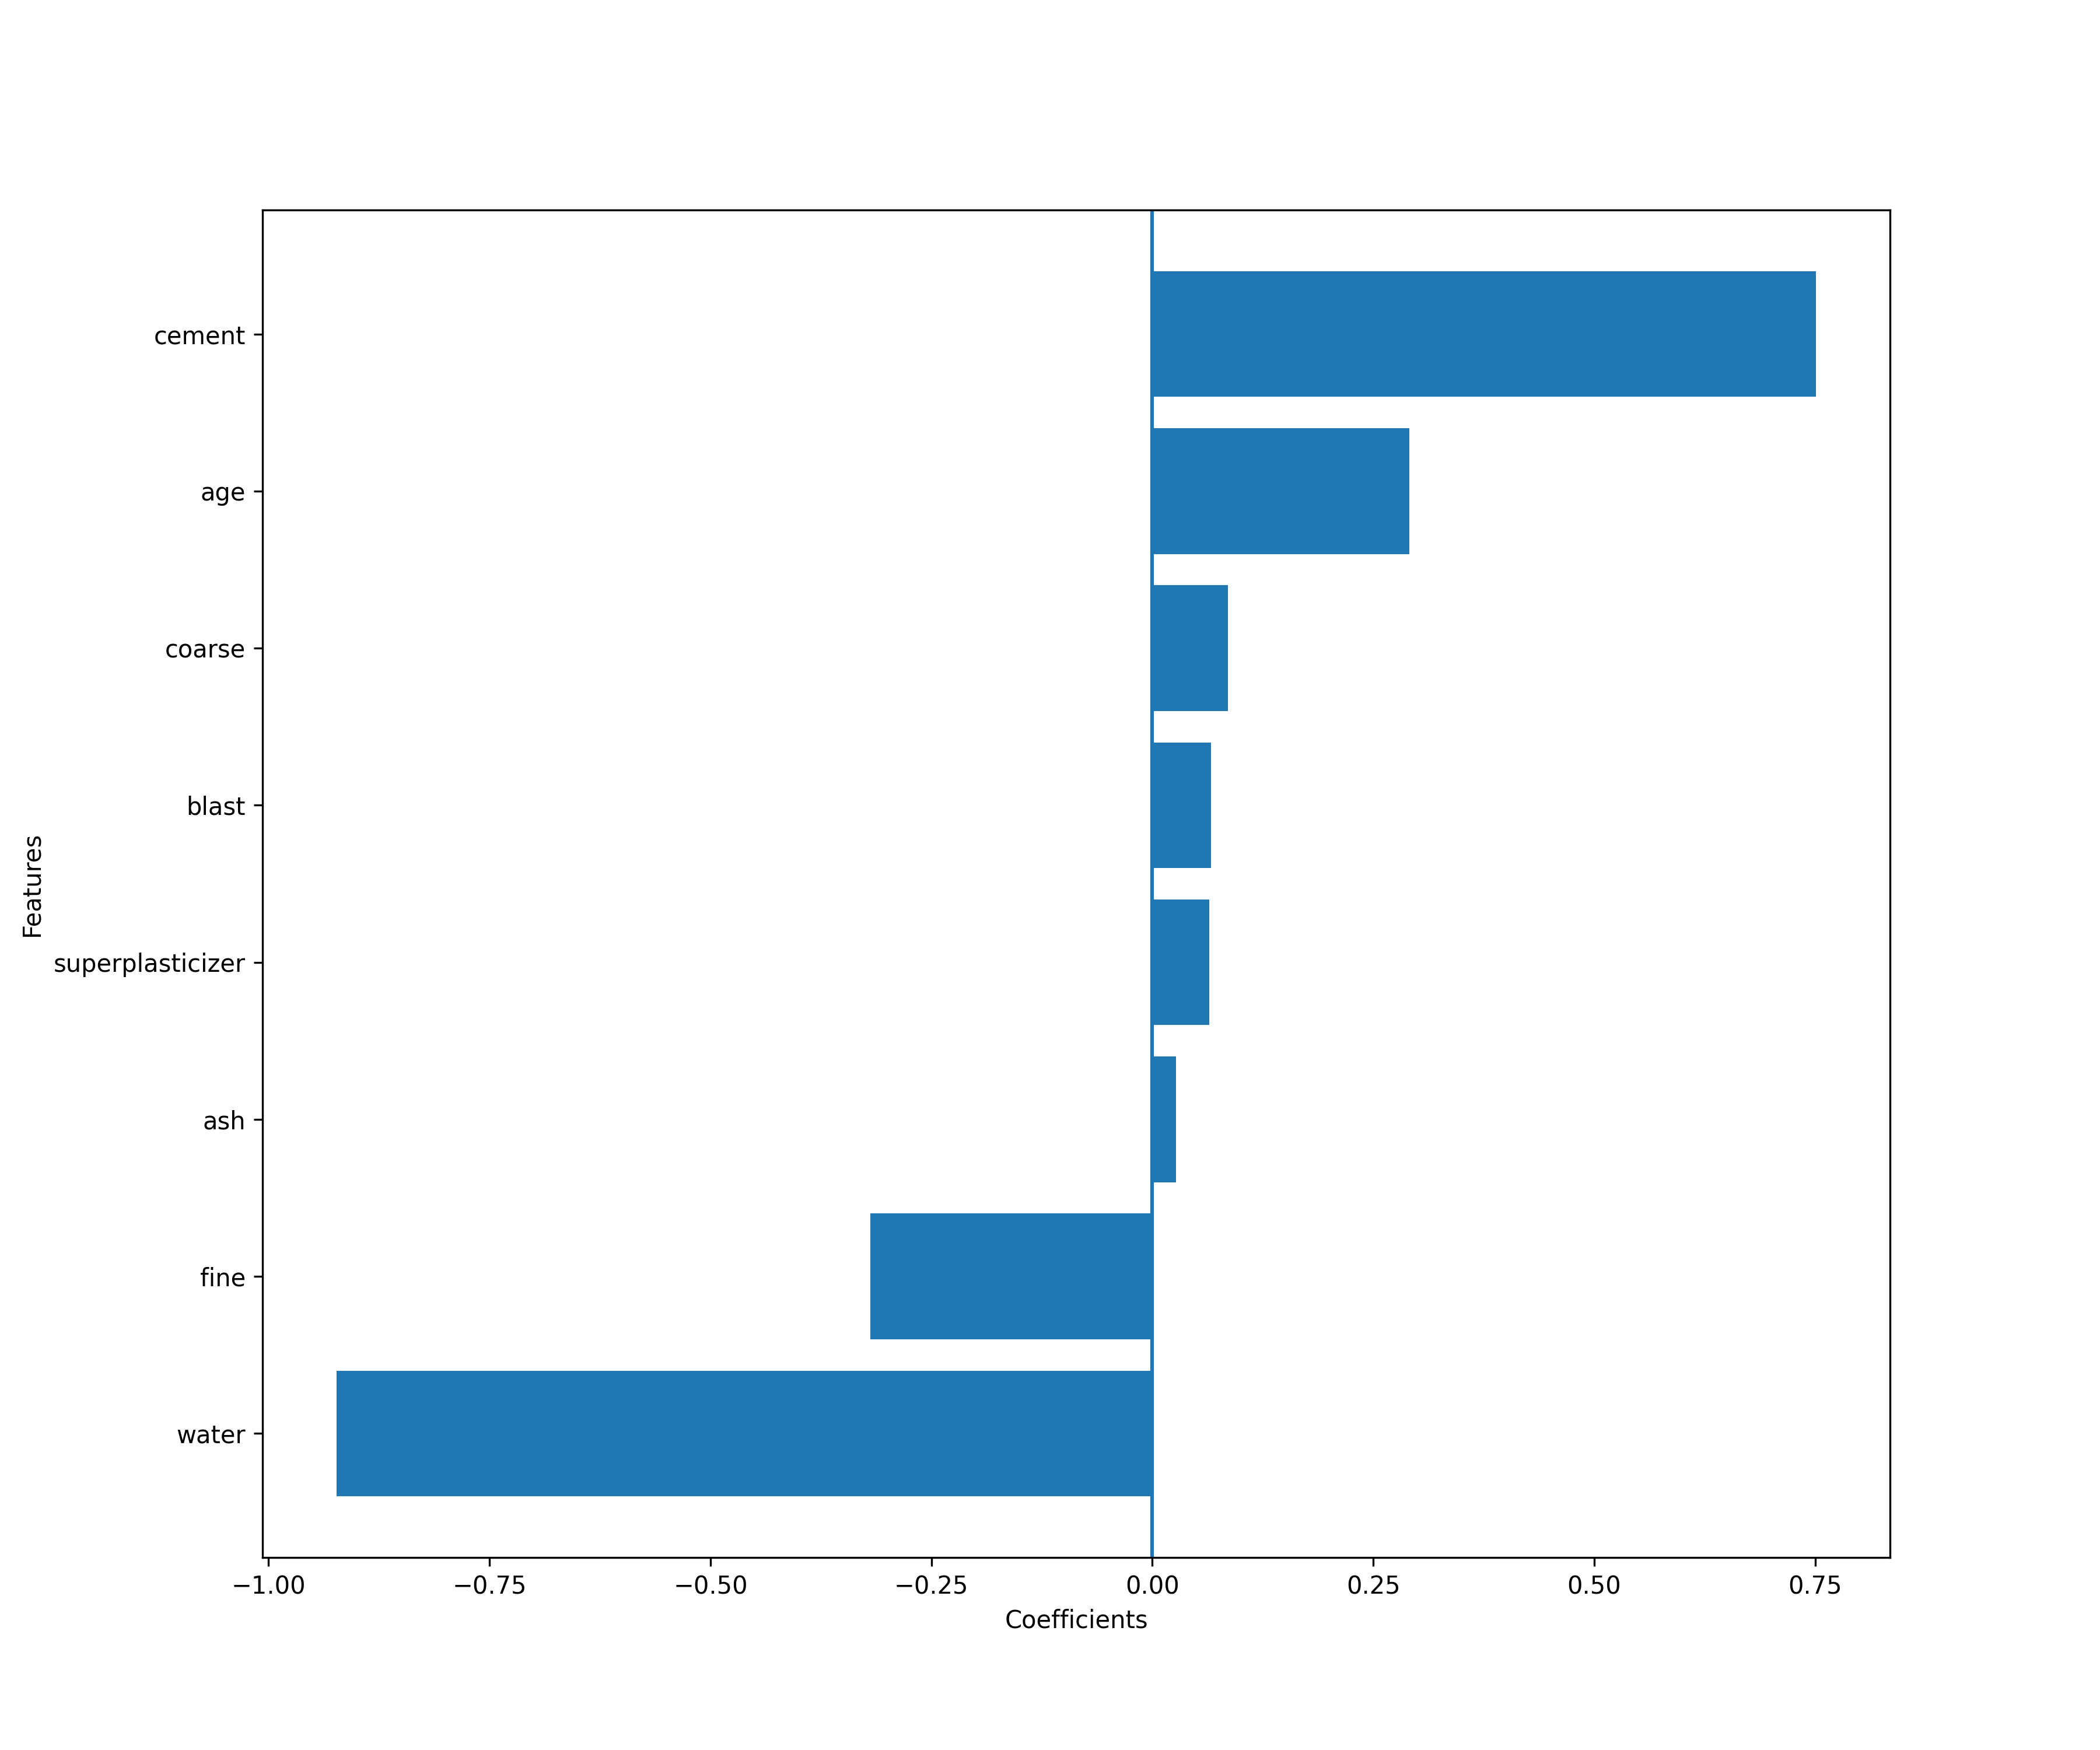
\includegraphics[width=1\textwidth]{../scripts/images/coef.png}
    Quelle: Eigene Darstellung, \ref{linreg}.
    \label{pic:coef}
\end{figure}

Die logarthimische Transformation der Merkmale hat dieses Problem bereits 
teilweise gelöst, indem sie die Skalierung der Daten angepasst hat und alle Merkmale auf eine einheitlichen Skala transformiert hat.
Daraus lassen sich erste Schlüsse der Merkmalsrelevanz ableiten. Im Vergleich zu allen anderen 
Koeffizienten tragen die Merkmale ash, superplasticizer, blast und coarse nur wenig zur abhängigen
Variable bei. 
Das obige Diagramm gibt Aufschluss über die Abhängigkeiten zwischen einem bestimmten Merkmal und der Zielvariablen, 
wenn alle anderen Merkmale konstant bleiben. Eine Erhöhung von cement führt zu einer Erhöhung der Druckfestigkeit. 
Im Gegensatz dazu führt eine Erhöhung von water zu einer Verringerung der Druckfestigkeit, immer unter der Vorraussetzung, das alle
anderen Merkmale konstant bleiben.

Im Anschluss an die Analyse der Koeffizienten des linearen Regressionsmodells wird 
die Feature Importance näher betrachtet. Ein bewährtes Verfahren zur Bestimmung der 
Feature Importance ist die sogenannte Permutation Feature Importance. 
Diese Methode misst die Veränderung im Vorhersagefehler des Modells nach der 
zufälligen Vertauschung der Werte eines bestimmten Merkmals. 
Ein Merkmal gilt als wichtig, wenn die Vertauschung seiner Werte den Modellfehler erhöht, 
da das Modell stark auf dieses Merkmal für seine Vorhersagen angewiesen ist. 
Umgekehrt wird ein Merkmal als unwichtig betrachtet, wenn die Vertauschung seiner Werte 
den Modellfehler unverändert lässt, da das Modell das Merkmal für seine Vorhersagen ignoriert \cite[S. 157]{Molnar_2022}. 

Abbildung \ref{pic:permutation} zeigt die Merkmalsrelevanz auf der Test- und Trainingsmenge 
anhand der Veränderung des mittleren quadratischen Fehlers des Modells:

\begin{figure}[!h]
    \caption{Permutation Feature Importance}
    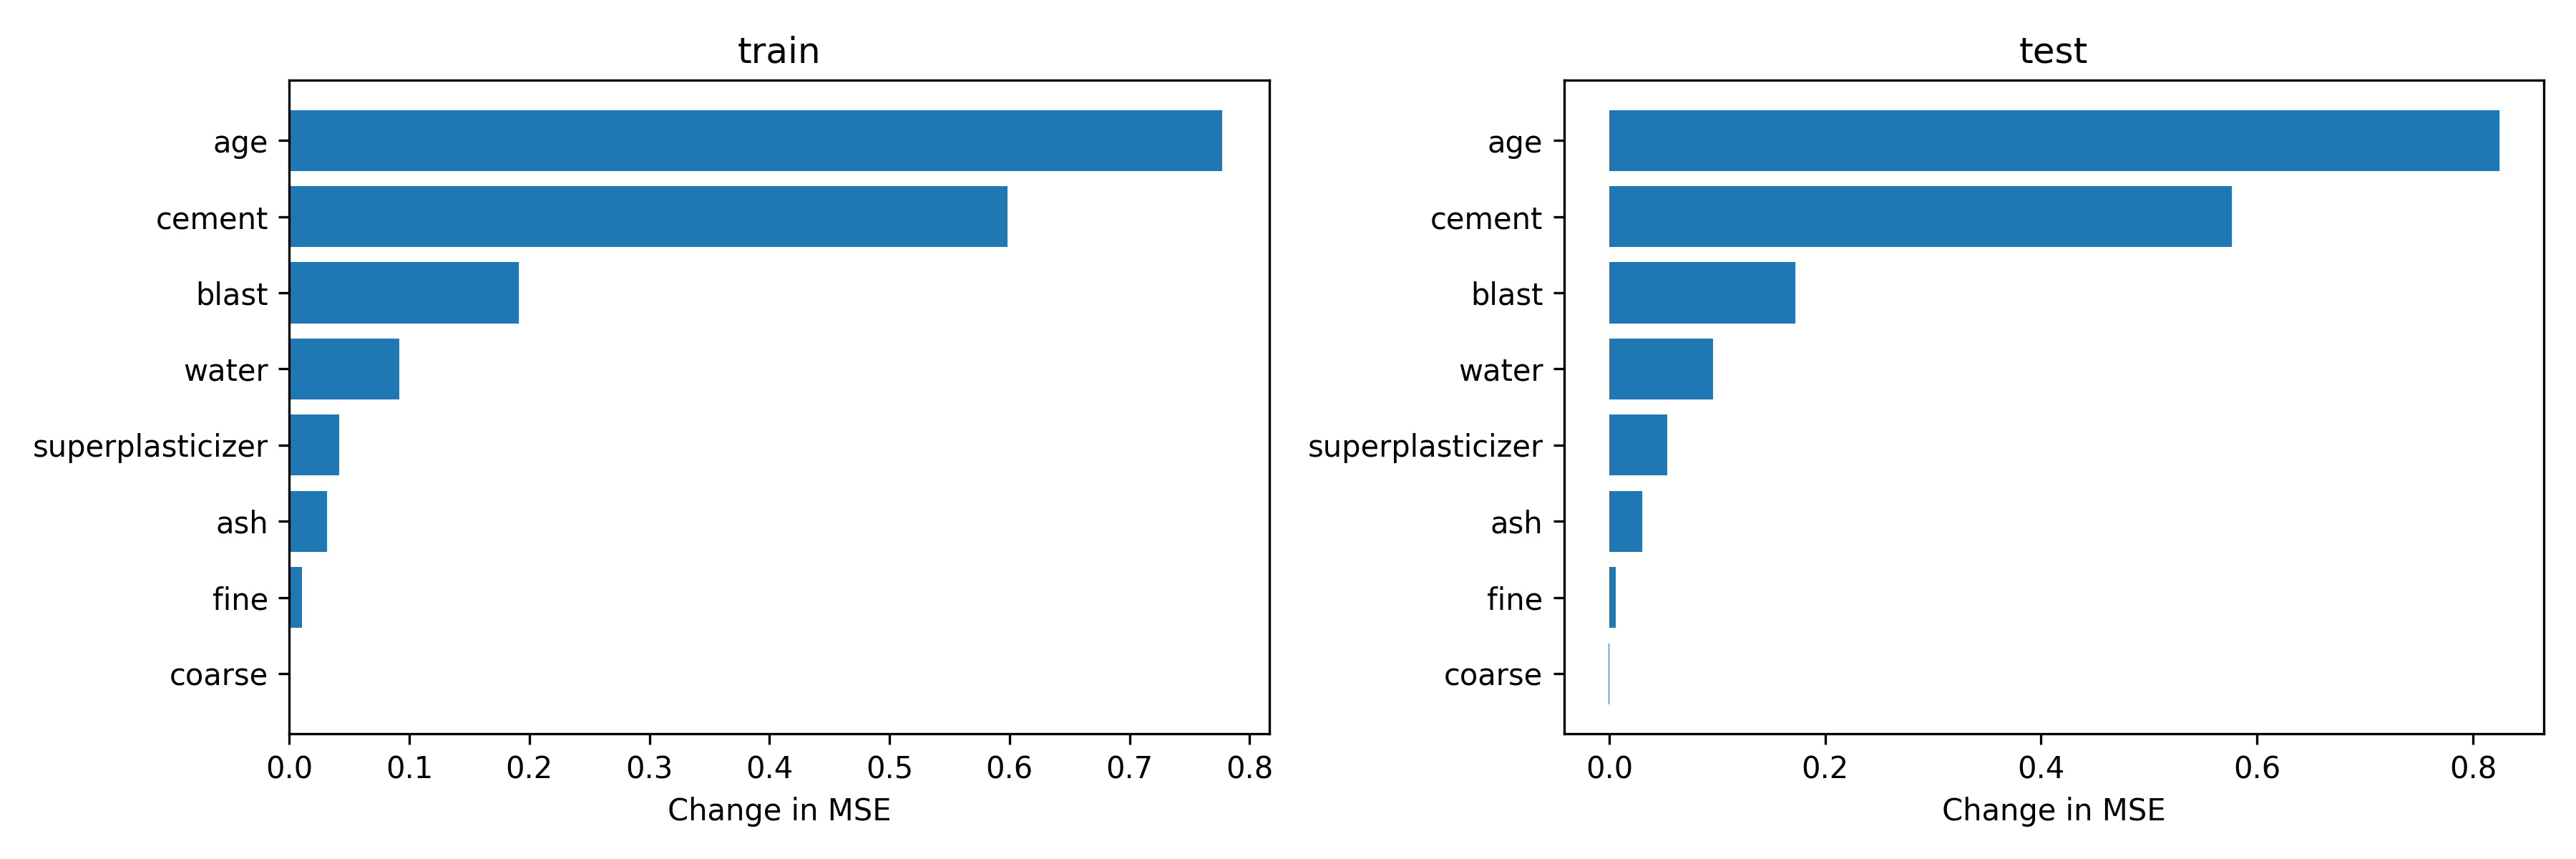
\includegraphics[width=1\textwidth]{../scripts/images/permutation_importance.png}
    Quelle: Eigene Darstellung, \ref{linreg}.
    \label{pic:permutation}
\end{figure}

Es ist festzustellen, dass die Merkmale coarse, fine und ash keine erhebliche Veränderung im mittleren quadratischen
Fehler des Modells hervorrufen und diese somit im Vergleich zu den anderen Merkmalen als eher irrelevant angesehen werden können.

\section{Interpretation mit SHAP}

Durch die Verwendung von SHAP-Werten wird 
es möglich, die Beiträge der einzelnen Merkmale zur Vorhersageleistung des Modells nicht nur 
auf globaler Ebene, sondern auch auf lokaler, individueller Ebene zu verstehen. 
SHAP-Werte berücksichtigen die Wechselwirkungen zwischen den Merkmalen und 
quantifizieren den Beitrag jedes Merkmals zur Abweichung der Prognose im Mittel. 
Dies ermöglicht eine präzisere Interpretation, da die SHAP-Werte den Einfluss 
eines Merkmals auf die Vorhersage unter Berücksichtigung aller anderen Merkmale anzeigen. 

\subsection{Lokale Interpretation}

Die lokale Interpretation konzentriert sich auf das Verständnis der Vorhersagen 
für eine einzelne Beobachtung aus dem Datensatz.

\begin{figure}[!h]
    \caption{SHAP Partial Dependence Plot}
    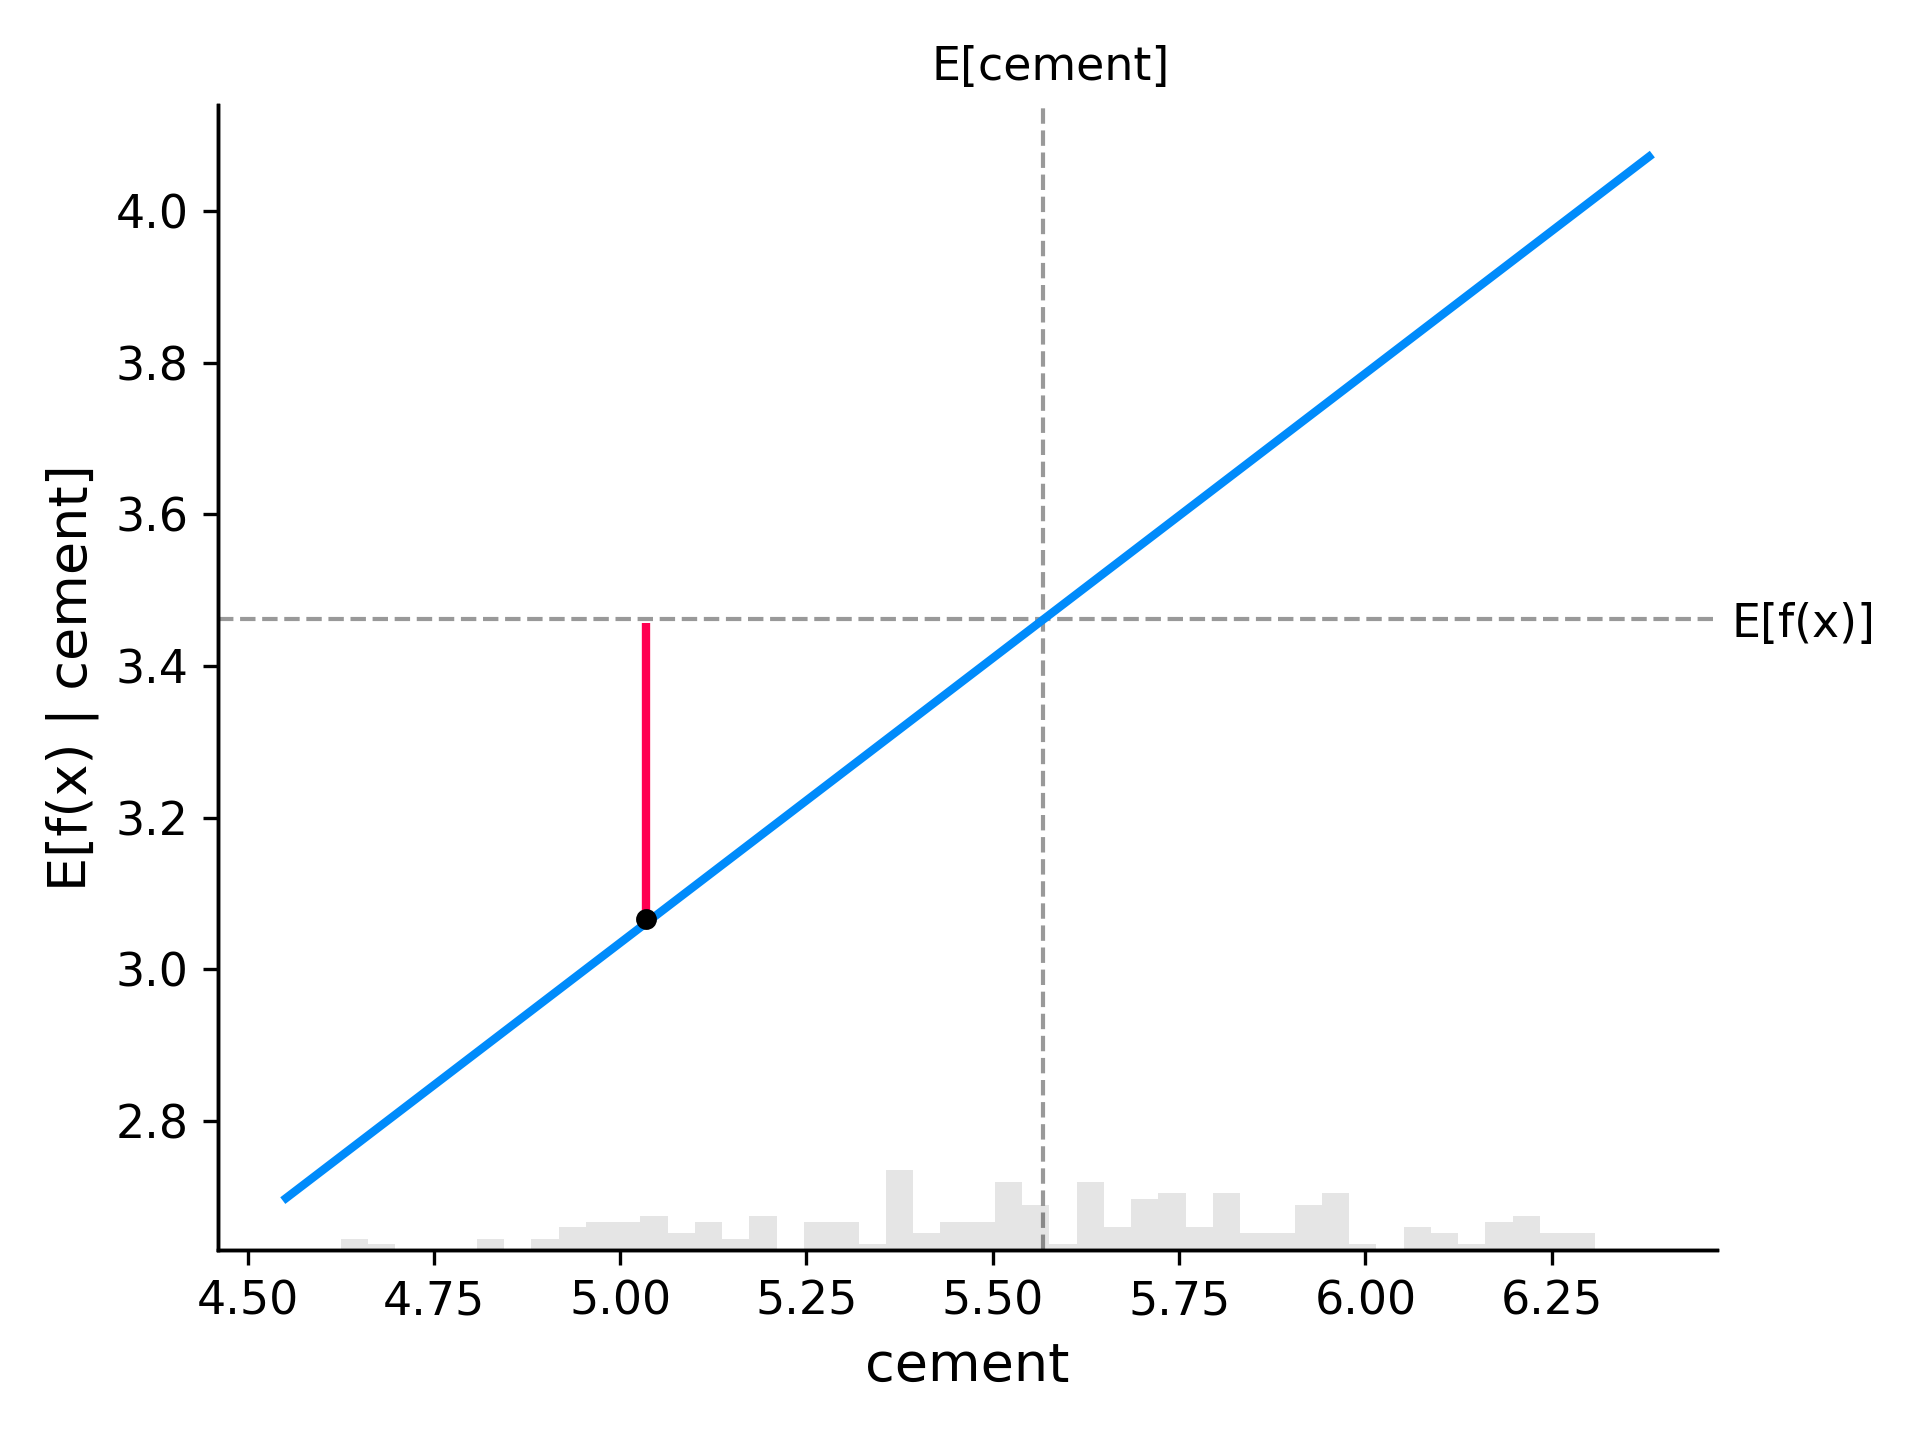
\includegraphics[width=1\textwidth]{../scripts/images/shap_dependence_plot.png}
    Quelle: Eigene Darstellung, \ref{linreg}.
    \label{pic:shap_dependence}
\end{figure}

Im Partial Dependence Plot der Abbildung \ref{pic:shap_dependence} wird die Beziehung zwischen 
dem Merkmal cement und der Zielvariable für die spezifische Beobachtung $x^{(0)}$ aus dem Datensatz visualisiert. 
Die blaue Linie im Diagramm repräsentiert die modellierte Abhängigkeit der Vorhersage vom Merkmal cement, 
unter Konstanthaltung aller anderen Merkmale. Der schwarze Punkt markiert die tatsächliche Ausprägung des 
Merkmals cement ($5.035$) für die betrachtete Beobachtung und die korrespondierende Vorhersage 
des linearen Regressionsmodells. Die rote Linie illustriert die marginale Abweichung der Vorhersage 
von der durchschnittlichen Modellprognose $\mathbb{E}[f(X)] = 3.421$, ausgehend vom beobachteten Wert von cement.

Die Anordnung des schwarzen Punktes entlang der funktionalen Beziehung gibt den spezifischen Wert 
von cement an und reflektiert, wie dieser Wert in den Kontext des gesamten Wertebereichs dieses Merkmals 
eingeordnet wird. Die vertikale Distanz zwischen der durchschnittlichen Vorhersage (dargestellt durch die horizontale 
gestrichelte Linie) und dem Punkt auf der funktionalen Abhängigkeit (blaue Linie) zeigt den Einfluss des Merkmals 
cement auf die individuelle Vorhersage im Vergleich zum Modellmittelwert. Dieser Einfluss verkörpert 
den marginalen Beitrag des Merkmals cement zur Prognoseabweichung für die ausgewählte Beobachtung.

Während der Partial Dependence Plot einen wertvollen Einblick in die Modellabhängigkeit von 
einzelnen Merkmalen bietet, ist für ein umfassendes Verständnis der Modellvorhersage eine ganzheitliche 
Betrachtung aller Merkmale notwendig. Der SHAP Waterfall Plot adressiert diese Notwendigkeit, 
indem er eine kumulative Darstellung aller marginalen Beiträge liefert. Jedes Merkmal wird in 
Form einer Sequenz von Beiträgen visualisiert, beginnend mit dem Basiswert der Vorhersage, welcher 
durch die Addition oder Subtraktion der individuellen Merkmalsbeiträge schrittweise zur finalen Vorhersage 
modifiziert wird.

\begin{figure}[!h]
    \caption{SHAP Waterfall Plot}
    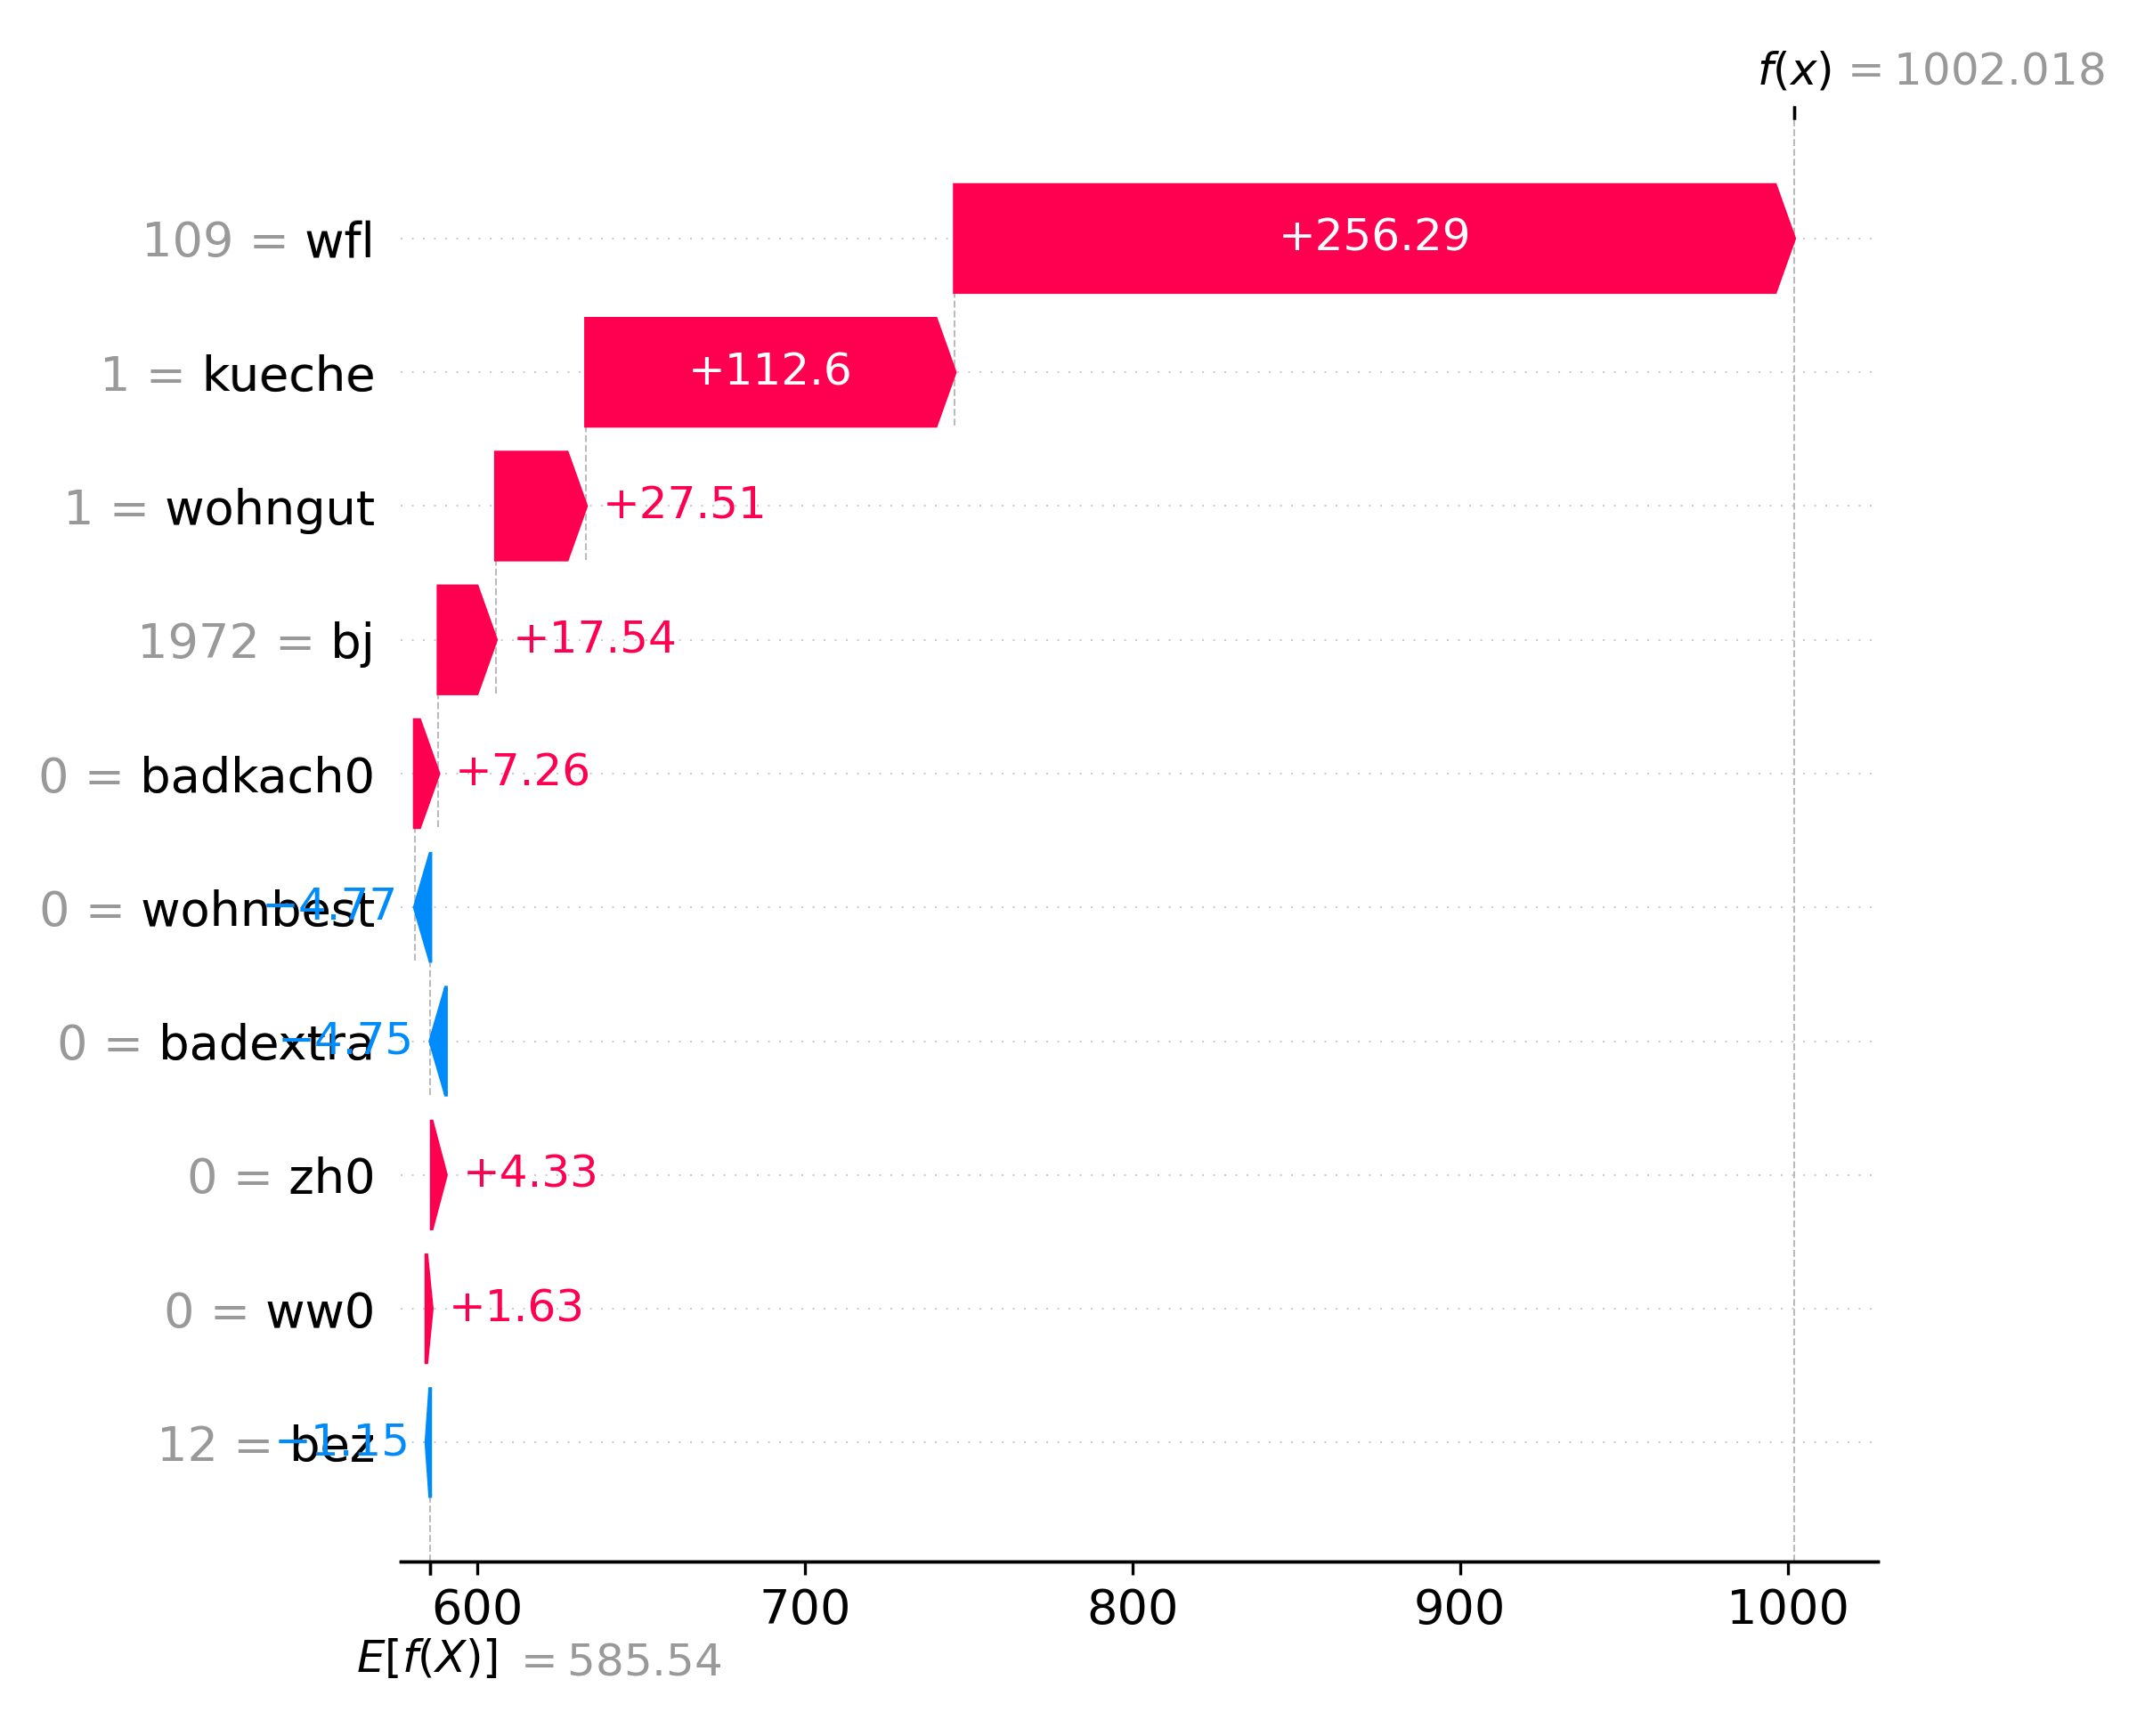
\includegraphics[width=1\textwidth]{../scripts/images/shap_waterfall_plot.png}
    Quelle: Eigene Darstellung, \ref{linreg}.
    \label{pic:shap_waterfall}
\end{figure}

In Abbildung \ref{pic:shap_waterfall} ist ein Waterfall Plot der ersten Beobachtung $x^{(0)}$ dargestellt, 
der die Zerlegung einer einzelnen Modellvorhersage zeigt. Der Plot beginnt mit dem Basiswert $\mathbb{E}[f(X)] = 3.421$, 
der durchschnittlichen Vorhersage des Modells. 

Von diesem Wert ausgehend, illustrieren die Balken, wie jede Merkmalausprägung – 
angezeigt durch die grauen Zahlen entlang der y-Achse – die Vorhersage $f(x_{j}^{(0)})$ beeinflusst. 
So steigert beispielsweise blast mit einem Wert von $4.982$ die Vorhersage um $+0.21$, 
wohingegen cement mit einem Wert von $5.035$ die Vorhersage um $-0.45$ verringert.

Rote Balken repräsentieren Merkmale, die die Vorhersage erhöhen, während blaue Balken solche 
darstellen, die sie senken. Die Größe jedes Balkens zeigt das Ausmaß des jeweiligen Beitrags, 
und die abschließende Vorhersage $f(x) = 3.257$ wird am Ende der Kette dieser Effekte erreicht. 

Kleine positive und negative Beiträge von Merkmalen wie fine ($6.713$), water ($5.188$), ash ($0$) und superplasticizer ($2.197$) 
zeigen, wie feingranulare Anpassungen der Merkmalsausprägungen die Vorhersage leicht erhöhen oder senken können.

Für die Beobachtung $x^{(0)}$ führt die kumulative Abweichung der Merkmal-Effekte 
vom Basiswert $\mathbb{E}[f(X)] = 3.421$ zu einem tatsächlichen Modelloutput von $f(x) = 3.257$, 
was eine Differenz von $-0.164$ zwischen der durchschnittlichen Vorhersage 
und der spezifischen Vorhersage für diese Beobachtung offenlegt. 
Diese Differenz entspricht der Summe aller SHAP-Werte für diese konkrete Beobachtung \cite[S. 52f]{Molnar_2023}.

Da die Zielgröße einer logarithmischen Transformation unterzogen wurde, muss diese für die Interpreation wieder rückgängig gemacht werden. 
Dies bedeutet, dass der tatsächliche erwartete Wert der Druckfestigkeit der Exponentialfunktion des prognostizierten Wertes entspricht, also $e^{3.421} \approx 30.60$ MPa. 
Dieser Rücktransformationsprozess ist notwendig, um die Modellprognosen in der ursprünglichen Skala der Zielvariablen zu interpretieren.
Dies gilt darüberhinaus sowhl für die einzelnen SHAP-Werte, als auch für die konkrete Vorhersage $f(x) = 3.257$. 
Die prognostizierte Durckfestigkeit für die Beobachtung $x^{(0)}$ beträgt folglich $e^{3.257} \approx 25.97$ MPa.

Dies ermöglicht eine detaillierte Analyse, wie das Modell zu einer bestimmten Vorhersage kommt, 
und hilft dabei, die Beiträge und Interaktionen zwischen verschiedenen Merkmalen zu verstehen.

Die lokale Interpretation mittels SHAP-Werten ermöglicht zwar eine präzise Erklärung 
der Modellvorhersagen für individuelle Beobachtungen, jedoch stellt sich bei einer 
solchen Betrachtung das Problem der fehlenden Generalisierbarkeit. 
Lokale Analysen können dazu führen, dass spezifische Merkmal-Kontributionen überinterpretiert werden, 
ohne die übergeordneten Muster und Einflüsse zu berücksichtigen, 
die das Modellverhalten im gesamten Datensatz charakterisieren. 
Eine globale Interpretation ist daher erforderlich, um die Konsistenz und Zuverlässigkeit 
des Modells über verschiedene Beobachtungen hinweg zu erfassen. 

\subsection{Globale Interpretation}

Der folgende Abschnitt widmet sich dieser globalen Sichtweise und untersucht, 
wie die Merkmalsa-Beiträge sich im Kontext des gesamten Datensatzes darstellen lassen.

\begin{figure}[!h]
    \caption{SHAP Beeswarm Plot}
    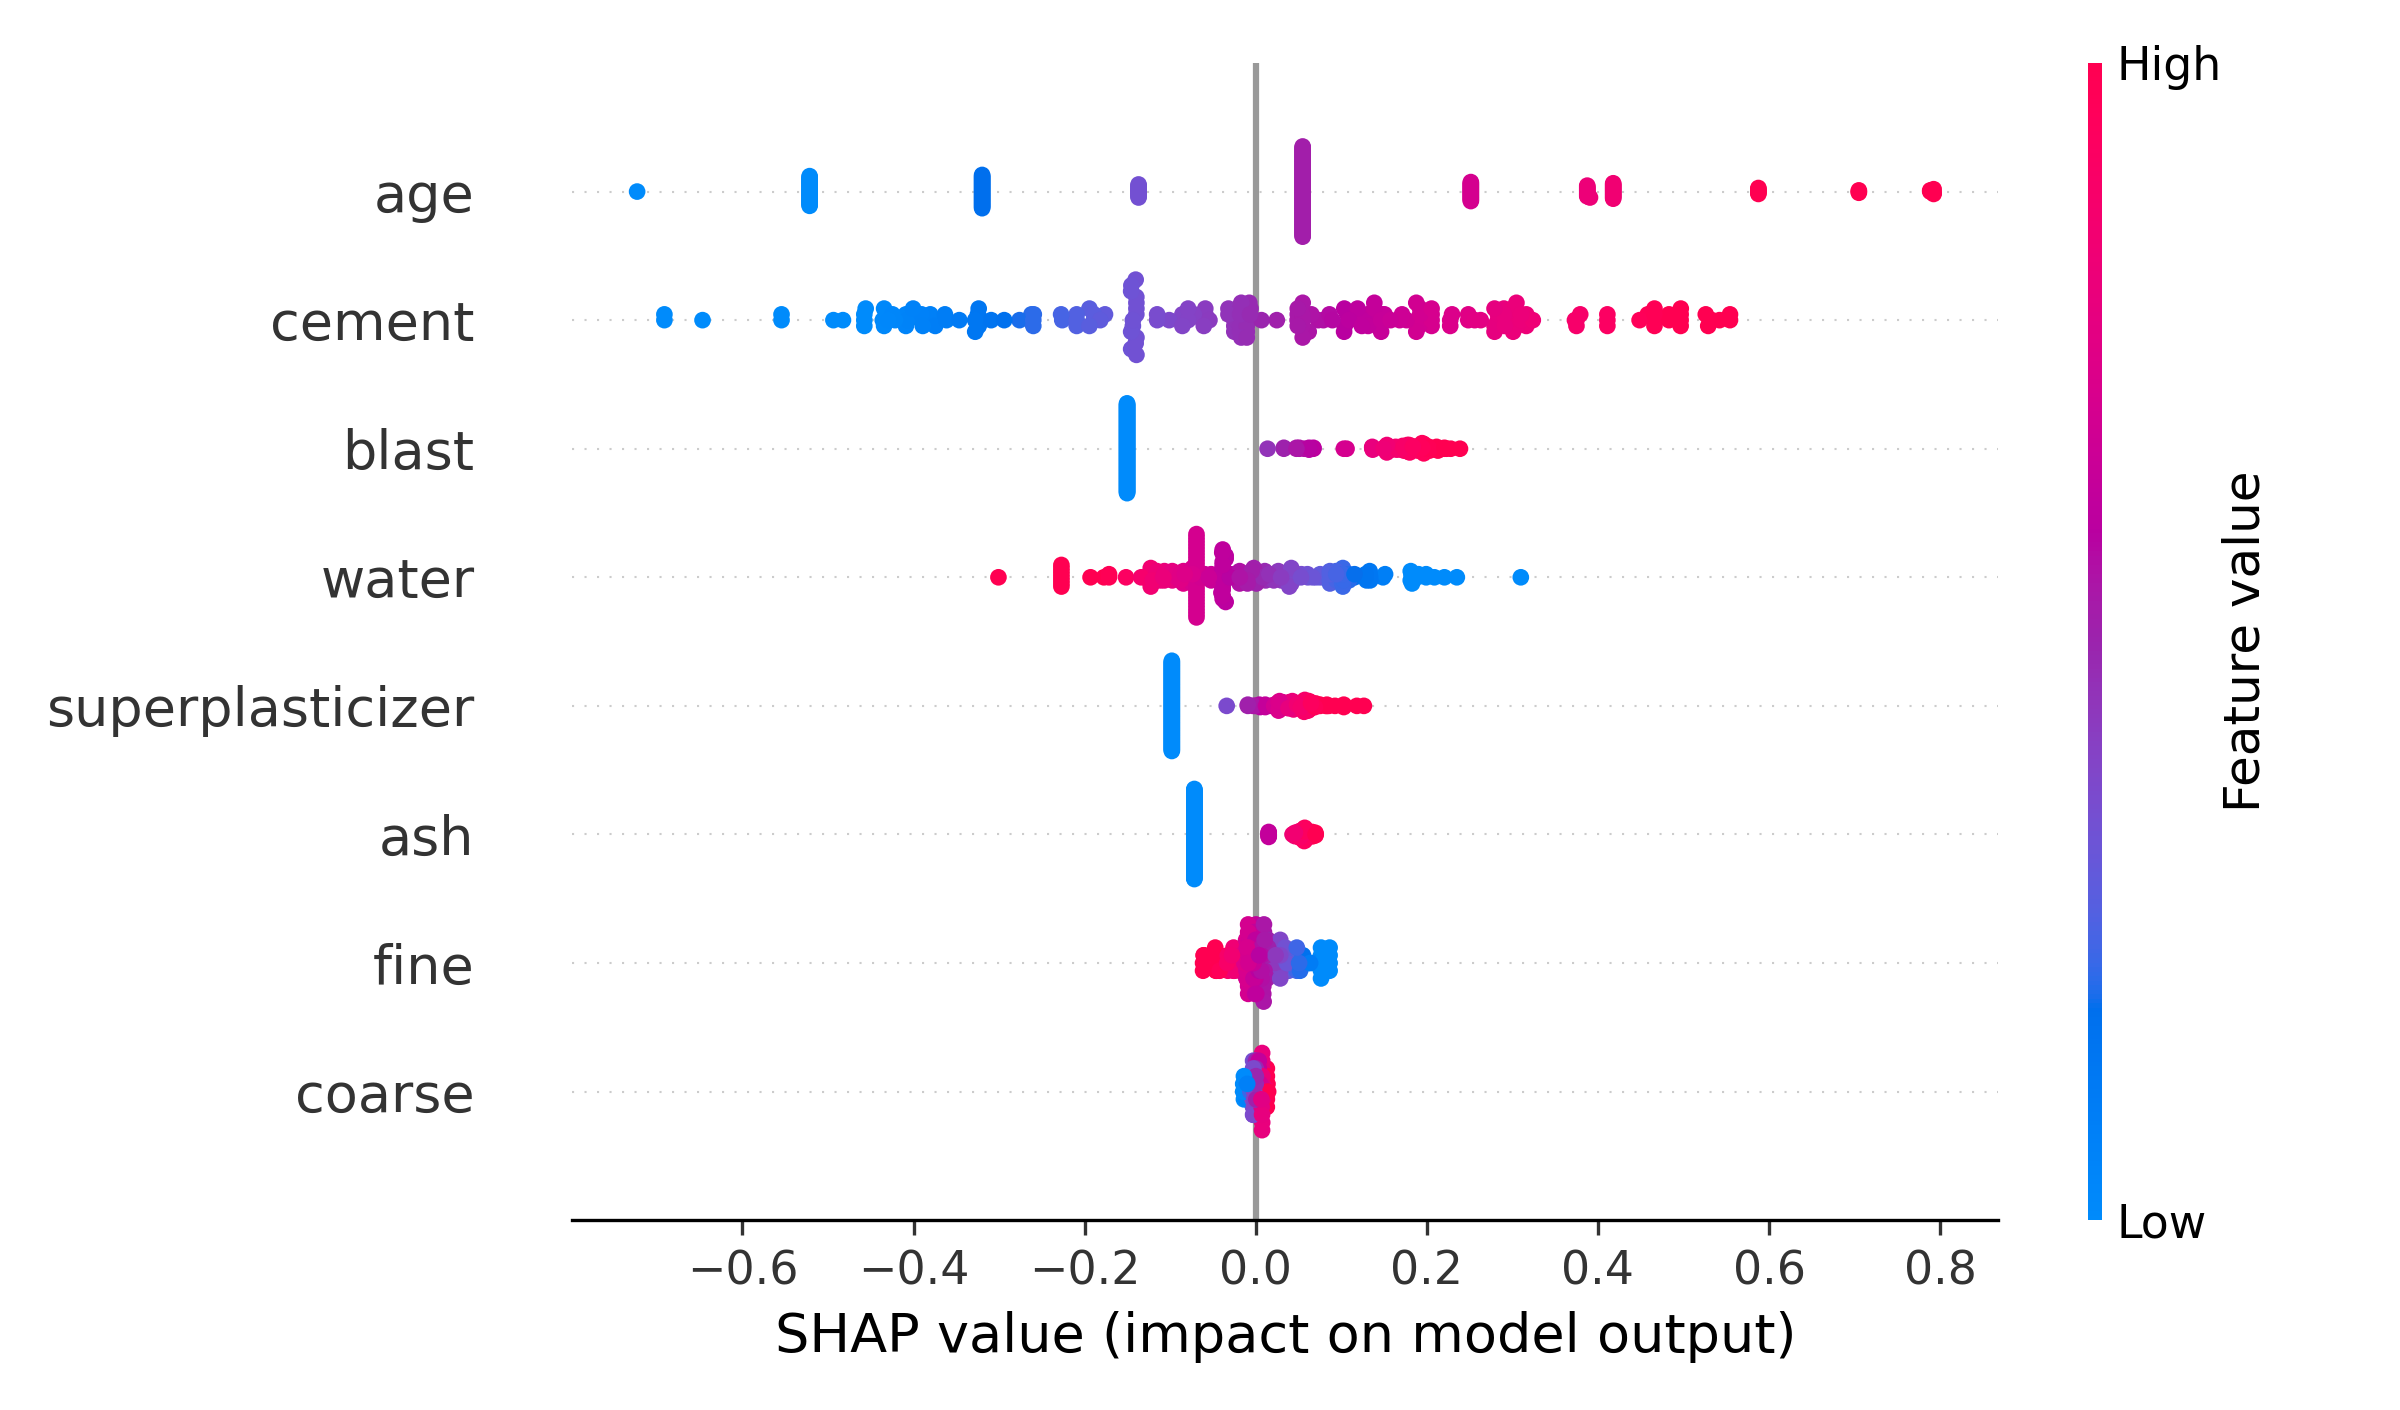
\includegraphics[width=1\textwidth]{../scripts/images/shap_beeswarm_plot.png}
    Quelle: Eigene Darstellung, \ref{linreg}.
    \label{pic:shap_beeswarm}
\end{figure}

Der SHAP Beeswarm Plot in Abbildung \ref{pic:shap_beeswarm} bietet eine globale 
Sicht auf die Modellvorhersagen, indem er die Verteilung der SHAP-Werte für jedes Merkmals 
über alle Beobachtungen hinweg darstellt. Jeder Punkt repräsentiert eine Beobachtung aus dem Datensatz.
Die Farbe der Punkte zeigt die Merkmalsausprägungen an: hohe Werte in Rot und niedrige Werte in Blau. 
Die Position auf der x-Achse gibt den Einfluss des Merkmals auf die Modellvorhersage an. 
Positive SHAP-Werte (rechts von der Nulllinie) zeigen eine Erhöhung der Vorhersage an, 
während negative Werte (links von der Nulllinie) eine Verringerung bedeuten. 

Das Merkmal age zeigt eine hohe Variabilität in seinem Einfluss auf die Modellvorhersage. 
Höhere Werte von age sind mit einer Zunahme der Vorhersage (positive SHAP-Werte) assoziiert, 
was durch die rechtsseitigen Punkte in der Grafik dargestellt wird. 
Niedrigere Werte führen hingegen zu einer geringeren Vorhersage, 
erkennbar an den linksseitigen Punkten. Diese Streuung der Punkte zeigt, 
dass die Auswirkung von age auf die Vorhersage stark von seiner quantitativen Ausprägung abhängt.

Diese Darstellung ermöglicht es, die Merkmale zu identifizieren, 
die den größten Einfluss auf das Modell haben und wie dieser Einfluss über 
unterschiedliche Beobachtungen variiert.

\begin{figure}[!h]
    \caption{SHAP Bar Plot}
    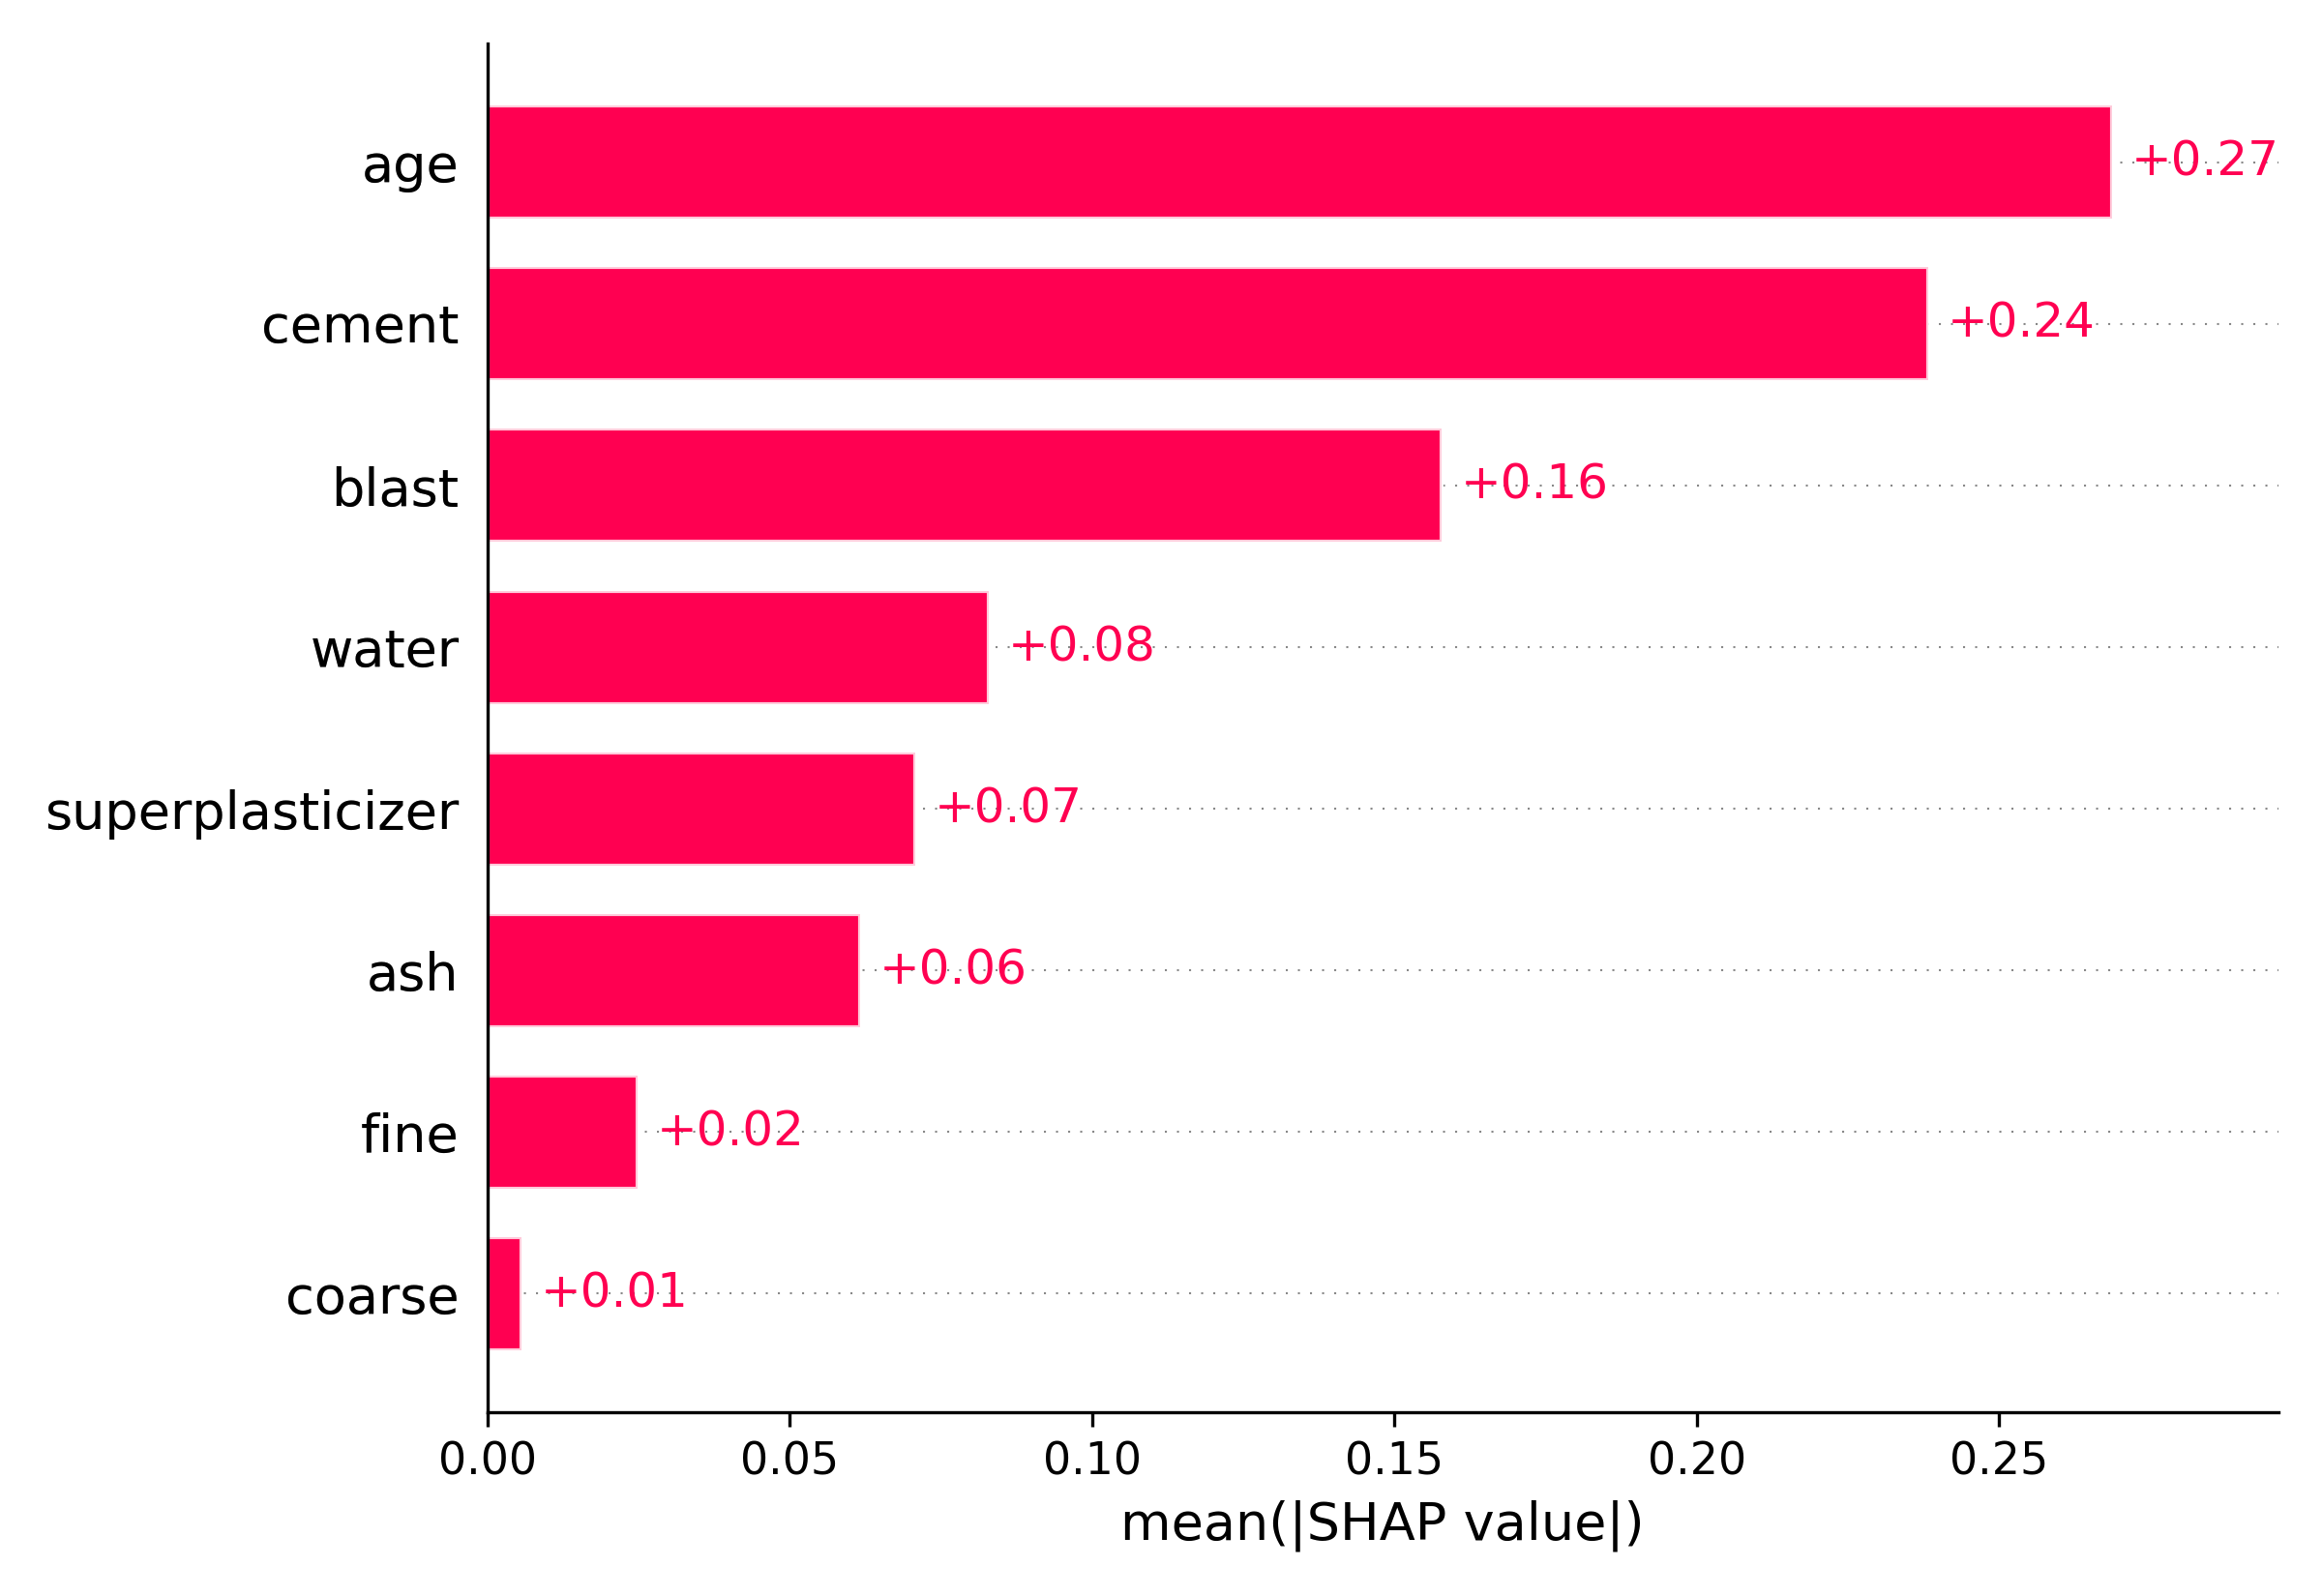
\includegraphics[width=1\textwidth]{../scripts/images/shap_bar_plot.png}
    Quelle: Eigene Darstellung, \ref{linreg}.
    \label{pic:shap_bar}
\end{figure}

Der SHAP Bar Plot in Abbildung \ref{pic:shap_bar} illustriert die durchschnittliche 
Auswirkung jedes Merkmals auf das Modell, gemessen an der absoluten Größe der SHAP-Werte 
über alle Beobachtungen hinweg. Die Balken zeigen die durchschnittlichen Beiträge der 
Merkmale zur Vorhersage: Je länger der Balken, desto größer ist der Einfluss des jeweiligen Merkmals. 
Hier ist das Merkmal age mit dem höchsten durchschnittlichen SHAP-Wert (+0.27) das einflussreichste 
Merkmal, was auf eine starke positive Beziehung zur Zielvariablen hinweist. Die weiteren Merkmale 
folgen in absteigender Reihenfolge ihrer Bedeutung.

Es fällt auf, dass eine Übereinstimmung in der Reihenfolge der Merkmalsrelevanz zwischen 
der Permutation Feature Importance aus Abbildung \ref{pic:permutation} und den SHAP-Werten aus Abbildung \ref{pic:shap_bar}
besteht, obwohl die zugrundeliegenden Interpretationen dieser beiden Methoden deutlich verschieden sind. 

Die Permutation Feature Importance konzentriert sich darauf, die Veränderungen im Vorhersagefehler des Modells, 
speziell den mittleren quadratischen Fehler, zu messen, die eintreten, wenn die Werte eines Merkmals zufällig vertauscht werden. 
Diese Methode gibt Aufschluss darüber, wie stark das Modell auf das jeweilige Merkmal für seine Vorhersagegenauigkeit angewiesen ist. 
Ein wesentliches Merkmal dieser Methode ist, dass sie nicht direkt die Wechselwirkungen zwischen den Merkmalen berücksichtigt. 
Sie zeigt vielmehr, wie wichtig ein Merkmal isoliert für die Gesamtleistung des Modells ist.

Im Gegensatz dazu bieten die SHAP-Werte einen tieferen Einblick in die Beiträge jedes Merkmals zur Vorhersageleistung des Modells. 
Sie quantifizieren den Einfluss eines Merkmals auf die Abweichung der Prognose vom Basiswert, also der durchschnittlichen Vorhersage des Modells. 
Hierbei wird nicht nur die individuelle Wichtigkeit jedes Merkmals hervorgehoben, sondern auch deren Wechselwirkungen mit anderen 
Merkmalen berücksichtigt. Diese Methodik ermöglicht es, sowohl eine globale als auch eine lokale Perspektive auf die Modellvorhersagen zu werfen. 
Während die globale Interpretation durchschnittliche Auswirkungen aller Merkmale aufzeigt, erlaubt die lokale Sichtweise, die Vorhersagen 
für einzelne Beobachtungen präzise zu erklären.

Diese unterschiedlichen Herangehensweisen und Interpretationen der Merkmalsrelevanz, einerseits durch die 
Permutation Feature Importance und andererseits durch die SHAP-Werte, verdeutlichen die Komplexität und die Tiefe der Analyse, 
die für ein umfassendes Verständnis von Vorhersagemodellen erforderlich ist. Beide Methoden ergänzen sich gegenseitig und tragen dazu bei, 
ein vollständigeres Bild der Dynamiken innerhalb des Modells zu zeichnen.

Shapley-Werte bieten für die Prognose der Druckfestigkeit von Beton einen signifikanten Vorteil, 
da sie eine gerechte Verteilung des Vorhersagebeitrags über alle Merkmale gewährleisten. 
Diese gerechte Verteilung ist eine der Kernstärken der 
Shapley-Werte, die sie von anderen Methoden abhebt.

Die Druckfestigkeit von Beton ist das Ergebnis einer komplexen Interaktion verschiedener 
Materialkomponenten und Eigenschaften wie Zementgehalt, Wasser-Zement-Verhältnis, 
Zuschlagstoffe und Alter des Betons. Jede dieser Komponenten trägt unterschiedlich 
zur Endfestigkeit bei, und ihre Effekte können nicht isoliert betrachtet werden, 
da sie interdependent sind. Hier ermöglichen Shapley-Werte eine faire und ausgewogene 
Zurechnung der Einflüsse jedes Merkmals auf die Vorhersage, indem sie die marginalen 
Beiträge jedes Merkmals unter Berücksichtigung aller möglichen Kombinationen von Merkmalen 
im Modell kalkulieren.

Andere Methoden, wie beispielsweise die Betrachtung von Regressionskoeffizienten, 
geben zwar Aufschluss über die Richtung und Stärke des Zusammenhangs zwischen Merkmalen 
und der Zielvariable, vernachlässigen jedoch die Interaktionseffekte zwischen den Merkmalen.

In der Praxis bedeutet dies für die Prognose der Druckfestigkeit von Beton, 
dass Shapley-Werte eine präzise Zuordnung der Einflussstärke jedes Bestandteils 
und Verarbeitungsmerkmals erlauben. Da die Festigkeit von Beton von einer Vielzahl von 
Faktoren abhängt, ermöglicht die granulare Aufschlüsselung der Shapley-Werte eine 
detailreiche Einsicht, welche Komponenten optimiert werden sollten, um die gewünschten 
Eigenschaften des Betons zu erreichen.

Im Kontext von industriellen Anwendungen und Forschung, wo Entscheidungen auf Grundlage 
der Modellvorhersagen getroffen werden, gewährleisten Shapley-Werte somit eine transparente 
und gerechtfertigte Grundlage. Dies ist nicht nur für die Entwicklung von Betonmischungen 
von Bedeutung, sondern auch für die Einhaltung von Bauvorschriften und die Gewährleistung 
der Sicherheit. Durch die Verwendung von Shapley-Werten kann die Forschung im Bereich 
der Materialwissenschaften fundierter und zielgerichteter gestaltet werden, was zu einer 
effizienteren und effektiveren Materialentwicklung führt.

Im abschließenden Kapitel dieser Arbeit werden die wichtigsten Erkenntnisse zusammengefasst 
und diskutiert.

